%\documentclass[landscape,a0b,final]{a0poster}
\documentclass[landscape,a0]{a0poster}
\pagestyle{empty}
\usepackage{tabularx}
\usepackage{amsmath}
\usepackage{amssymb}
\usepackage{pst-all}
\usepackage{epsfig}
\usepackage{wallpaper}
\usepackage{url}
\usepackage[latin1]{inputenc}
\usepackage{multirow}


\renewcommand{\vec}[1]{\mathbf{#1}}

% space of the real numbers
\newcommand{\R}{\ensuremath{\mathbb{R}}}
% space of the integer numbers
\newcommand{\Z}{\ensuremath{\mathbb{Z}}}
% Digitization process of step h (1)
\newcommand{\Dig}[1]{\ensuremath{\mathrm{Dig}_{#1}}}
% Family of shape
\newcommand{\SF}[0]{\ensuremath{\mathbb{F}}}
% Topological boundary of X (1).
\newcommand{\TB}[1]{\ensuremath{\partial #1}}
% Discrete geometric estimator of G (1)
\newcommand{\DGE}[1]{\ensuremath{E_{#1}}}
% Reference shape of digital object O (1) with grid step $h$ (2).
\newcommand{\RS}[2]{\ensuremath{R_{#1,#2}}}

% Digital contour.
\newcommand{\DC}{\ensuremath{C}}
% Continuous contour.
\newcommand{\CC}{\ensuremath{\mathcal{C}}}
% A point indexed by i (1) on the digital contour.
\newcommand{\PT}[1]{\ensuremath{\DC_{#1}}}
% A sequence of points indexed by i (1) on the digital contour.
\newcommand{\PTS}[2]{\ensuremath{\DC_{#1,#2}}}
% Predicate stating that the digital curve is a segment between indices 1 and 2
\newcommand{\SPRED}[2]{\ensuremath{S(#1,#2)}}
% ET logique
\newcommand{\AND}[0]{\ensuremath{\wedge}}
% OU logique
\newcommand{\OR}[0]{\ensuremath{\vee}}

% Tangent direction mapping of curve C (1)
\newcommand{\TGT}[1]{\ensuremath{\theta_{#1}}}
% Integral of squared curvature of curve C (1)
\newcommand{\ISC}[1]{\ensuremath{J[#1]}}
% Smallest possible tangent direction at constraint l (1)
\newcommand{\MinTD}[1]{\ensuremath{a_{#1}}}
% Largest possible tangent direction at constraint l (1)
\newcommand{\MaxTD}[1]{\ensuremath{b_{#1}}}
% Unknown tangent direction at constraint l (1)
\newcommand{\UnkTD}[1]{\ensuremath{t_{#1}}}

% ideal multiscale criterion
\newcommand{\IMSC}[2]{\ensuremath{\mu_{#1}(#2)}}
% multiscale profile
\newcommand{\MSP}[2]{\ensuremath{\mathcal{P}_{#1}(#2)}}
% threshold flat/curve
\newcommand{\CThreshold}[0]{\ensuremath{t_{f/c}}}
% threshold noise
\newcommand{\NThreshold}[0]{\ensuremath{t_{m}}}
% noise level
\newcommand{\NL}[0]{\ensuremath{\nu}}
% slope linear regression 
\newcommand{\SLR}[2]{\ensuremath{\theta_{#1}}}





% Pencil of maximal segments around a point.
\newcommand{\PE}[1]{\ensuremath{{\mathcal P}(#1)}}
% Tangent orientation of the maximal segment.
\newcommand{\TO}[1]{\ensuremath{\theta_#1}}
% lambda function for interpolation.
\newcommand{\LF}{\ensuremath{\lambda}}
% \lambda-MS tangent orientation.
\newcommand{\LTO}[1]{\ensuremath{\hat{\theta}(#1)}}
% \lambda-MS tangent orientation variation.
\newcommand{\LTOP}[1]{\ensuremath{\hat{\theta}'(#1)}}

%\definecolor{rougeSW_}{rgb}{0.968627,0.011765,0.015686}
\definecolor{darkgreen}{rgb}{0.0,0.6,0.0}
\definecolor{lightblue}{rgb}{0.5,0.5,1.0}
\definecolor{magenta}{rgb}{1.0,0.0,1.0}
\newcommand{\alertred}[1]{{\color{red}#1}}
\newcommand{\Cb}[1]{{\color{blue}#1}}
\newcommand{\Cdg}[1]{{\color{darkgreen}#1}}
\newcommand{\textmagenta}[1]{{\color{magenta}#1}}
\newcommand{\Implies}{{\ensuremath{\Rightarrow}}}

\newcommand{\Refs}[1]{{\color{lightblue}#1}}
\newcommand{\Cite}[1]{\Refs{[#1]}}
\newcommand{\Etal}{{\em et al.}}
\newtheorem{remark}{Remarque}
% Digitization process of step h (1)
\newcommand{\DigGh}[2]{\ensuremath{\mathrm{Dig}_{#2}(#1)}}
\newcommand{\BigT}{\ensuremath{\Theta}}
\newcommand{\BigO}{\ensuremath{O}}

\newcommand{\TAN}[0]{\ensuremath{\theta}}
% Position estimator
\newcommand{\EPOS}[0]{\ensuremath{\hat{{x}}}}
% Convexity Position estimator 
\newcommand{\ECONVPOS}[0]{\ensuremath{\hat{x}^\mathrm{conv}}}
% tangent estimator base MS.
\newcommand{\ETANMS}[0]{\ensuremath{\hat{\TAN}^{\text{MS}}}}
% tangent estimator base arete du CDP.
\newcommand{\ETANEDGE}[0]{\ensuremath{\hat{\TAN}^{\text{conv}}}}
% estimateur de longueur elementaire d'un surfel (1) sur le bord discretise de X(2) de pas h(3).



\newcounter{posterPartNum}
\setcounter{posterPartNum}{0}



\definecolor{Rouge}{rgb}{1.0, 0.0, 0.0}
\definecolor{RougeSombre}{rgb}{0.8, 0.0, 0.0}
\definecolor{Vert}{rgb}{0.0, 1.0, 0.0}
\definecolor{VertSombre}{rgb}{0.0, 0.5, 0.0}
\definecolor{Bleu}{rgb}{0.0, 0.0, 1.0}
\definecolor{BleuSombre}{rgb}{0.0, 0.0, 0.8}
\definecolor{PartColor}{rgb}{0.0, 0.5, 0.0}

\newrgbcolor{lcolor}{0. 0. 0.80}
\newrgbcolor{gcolor1}{1. 1. 1.}
\newrgbcolor{gcolor2}{.80 .80 1.}



\renewcommand{\vec}[1]{\overrightarrow{\strut #1}}

\newcommand{\pd}[2]{\frac{\partial #1}{\partial #2}}

\newlength{\pfLeft}
\newlength{\pfRight}
\newlength{\pfTop}
\newlength{\pfBottom}

%% Pour faire des jolis itemize
\newlength{\svg}
\newenvironment{posterDescription}
{
	\begin{list}{}
	{
		\setlength{\leftmargin}{1.0cm}
		\setlength{\labelsep}{0.1cm}
		\setlength{\labelwidth}{1.0cm}
		\setlength{\itemindent}{0cm}
		\setlength{\listparindent}{0cm}
		\setlength{\itemsep}{0.1cm}
	}
}
{
	\end{list}
}







\newenvironment{colonne}[1]{
\begin{minipage}[t]{#1\textwidth}
  \begin{center}}{
  \end{center}
  \end{minipage}}




\newcommand{\pbox}[4]{
\psshadowbox[#3]{
\begin{minipage}[t][#2][t]{#1}
#4
\end{minipage}
}}






\newenvironment{poster}[1]
{ 
  \begin{center}
    {\Huge \bf \sffamily  #1}
    %	\posterPartSeparator
  \end{center}
}


\setlength{\wpYoffset}{-2.5cm}


\begin{document}



%----------------------------------------------------------------
%
%     Image de fond
%\wpYoffset{0.2cm}

\CenterWallPaper{1.0}{./Logos/DGtalLogoFond2.eps}	

\sffamily
\newrgbcolor{lightblue}{0. 0.2 0.20}
\newrgbcolor{white}{1. 1. 1.}
\newrgbcolor{whiteblue}{.80 .80 1.}






\begin{poster}{

\begin{colonne}{0.98}
%\psframe[linewidth=2mm,framearc=0.2,linecolor=lightblue,framesep=1em](-47,3)(47,-12.5)
\begin{center}
\vspace{-1.5cm}
\centering \rput(4cm,1cm){
\includegraphics[width=8cm]{Logos/DGtalLogo.eps}} \hskip 10cm Digital Geometry Tools and Algorithms \\
\rput(-40cm,1cm){\psline(0,0)(80cm,0)}
\center \rput(0cm,-0cm){\includegraphics[width=14cm]{Logos/logoDGCI2.eps}} \\
\vspace{2cm}
{\LARGE \url{http://liris.cnrs.fr/dgtal}}

\center \Large{LORIA 6-8 avril 2011}  

\rput(-30cm,1cm){\psline(0,0)(60cm,0)}
\vspace{4.5cm}

\end{center}


\end{colonne}
}

%-------------------------------------------------------------------------------
% Colonne 1
%-------------------------------------------------------------------------------
%\vskip 4cm
\begin{colonne}{0.32}

\begin{minipage}[t]{\textwidth}
\section{DGtal: a software library for the discrete geometry community}

\subsection{Objectives}

\begin{itemize}
\item to make easier discrete geometry for the neophyte (student, researcher from another field, \ldots)
\item to test quickly new ideas, with objective comparison wrt
  existant works
\item to make easier the implementation of demonstrators
\item to help spread our research results to other domains
\item to pursue a federative project
\item \ldots
\end{itemize}

\subsection{Main features}

\begin{itemize}
\item to define digital objects in arbitrary dimension
\item to propose algorithms for topological and geometric analysis
\item to facilitate image analysis with data structures
\item to provide I/O mechanisms and visualization tools
\end{itemize}


\subsection{Philosophy}

 \begin{itemize}
 \item {\bf \color{red} Genericity} and {\bf \color{red} efficiency}
 \item C++ library, concepts, generic programming with templates   
 \item open-source, LGPL or GPL with restrictions
 \item user friendly, not necessarily kernel-developer friendly
 \end{itemize}

\subsection{A collaborative effort}
\smallskip

\begin{center}
\begin{tabular}{ccccc}

\includegraphics[width=0.16\textwidth]{Images/liris-logo.eps}&

\includegraphics[width=0.16\textwidth]{Images/lama-logo.eps}&

\includegraphics[width=0.16\textwidth]{Images/loria-logo.eps}&

\includegraphics[width=0.16\textwidth]{Images/gipsa-logo.eps}&

\includegraphics[width=0.16\textwidth]{Images/greyc-logo.eps}\\
LIRIS (Lyon)&
LAMA (Chamb�ry)&
LORIA (Nancy)&
Gipsa-lab (Grenoble)&
GREYC (Caen)\\
\end{tabular}
\end{center}

\subsection{The current DGtal team}
\smallskip


\begin{itemize}
\item David Coeurjolly (LIRIS): infrastructure, kernel, images,
  volumetric geometry
\item Jacques-Olivier Lachaud (LAMA): kernel, topology, 2D display (board)
\item Bertrand Kerautret (LORIA): contours, 3D viewer
\item Tristan Roussillon (LIRIS): 2D geometry
\item Guillaume Damiand (LIRIS): kernel
\item S�bastien Fourey (GREYC): kernel, board
\item Isabelle Sivignon (Gipsa-lab): DSS
\end{itemize}

\end{minipage}

\end{colonne}
\hfill
%-------------------------------------------------------------------------------
% Colonne 2
%-------------------------------------------------------------------------------
\begin{colonne}{0.32}

\begin{minipage}[t]{\textwidth}
\section{Structure}
\begin{center}
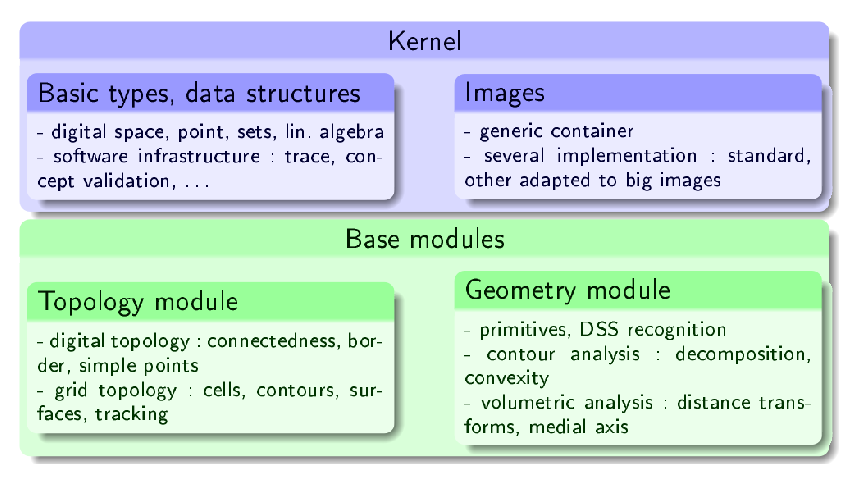
\includegraphics[width=0.7\textwidth]{Images/structure.eps}
\end{center}

\section{Features and examples}

\subsection{Generic spaces, domain, sets, etc}

\begin{itemize}
\item arbitrary spaces, spanning iterators, adaptative type of sets
\end{itemize}

\begin{center}
\begin{tabular}{cc}
\framebox{%
  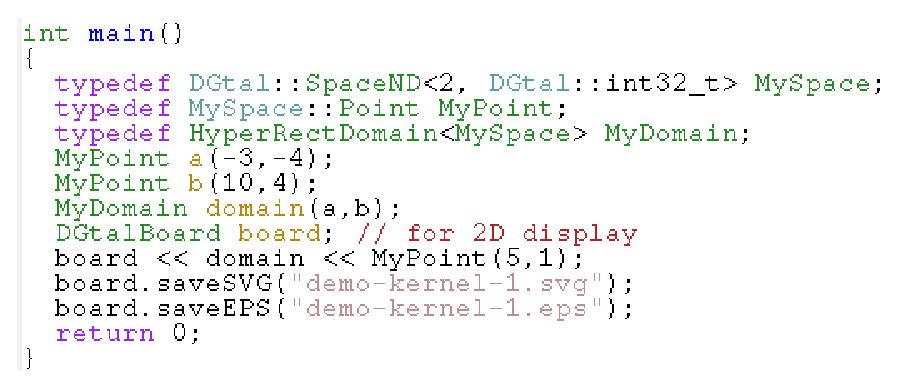
\includegraphics[width=0.45\textwidth]{Images/code-demo-kernel-1.eps}%
}&
\framebox{%
  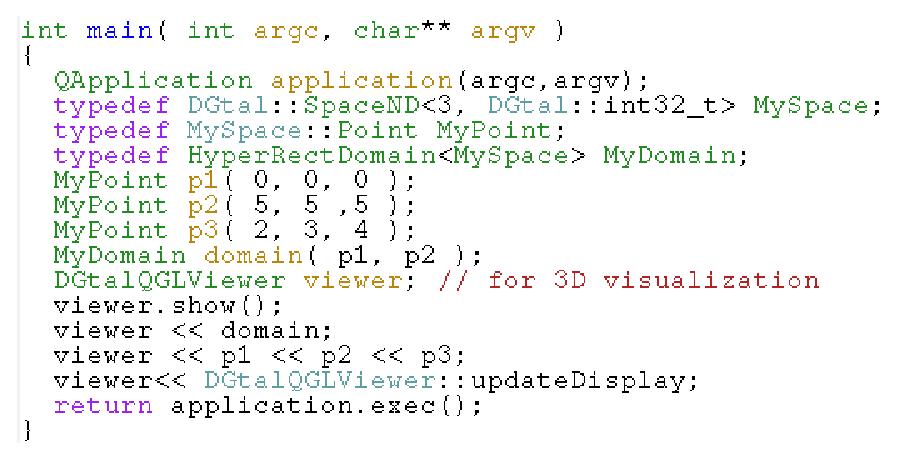
\includegraphics[width=0.45\textwidth]{Images/code-demo-kernel-2.eps}%
}\\
\framebox{%
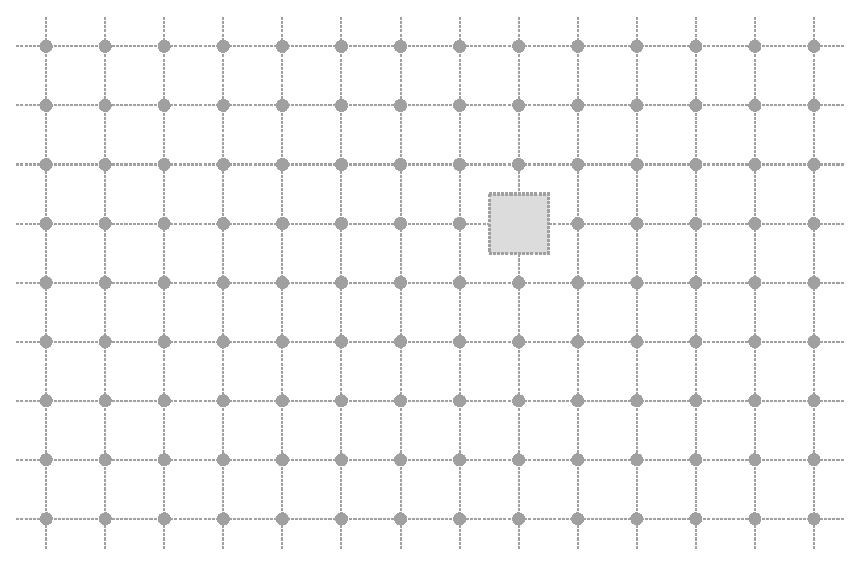
\includegraphics[width=0.35\textwidth]{Images/demo-kernel-1.eps}%
}&
\framebox{%
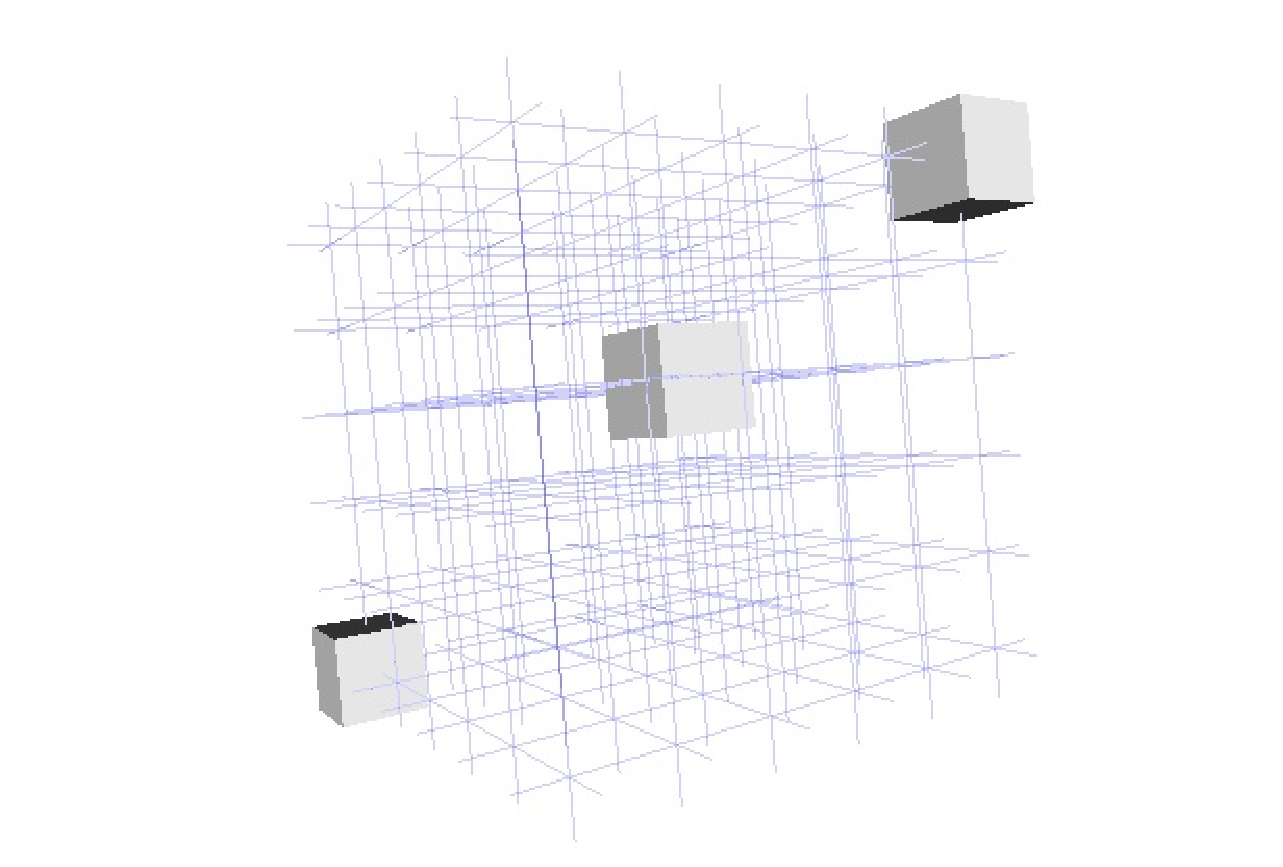
\includegraphics[width=0.35\textwidth]{Images/demo-kernel-2.eps}%
}\\
\end{tabular}
\end{center}

\subsection{Generic images, adaptative containers}

\begin{itemize}
\item several image containers (vector, hashtree), ITK backend
\end{itemize}

\begin{center}
\begin{tabular}{c@{\hskip 4cm}c}
\framebox{%
  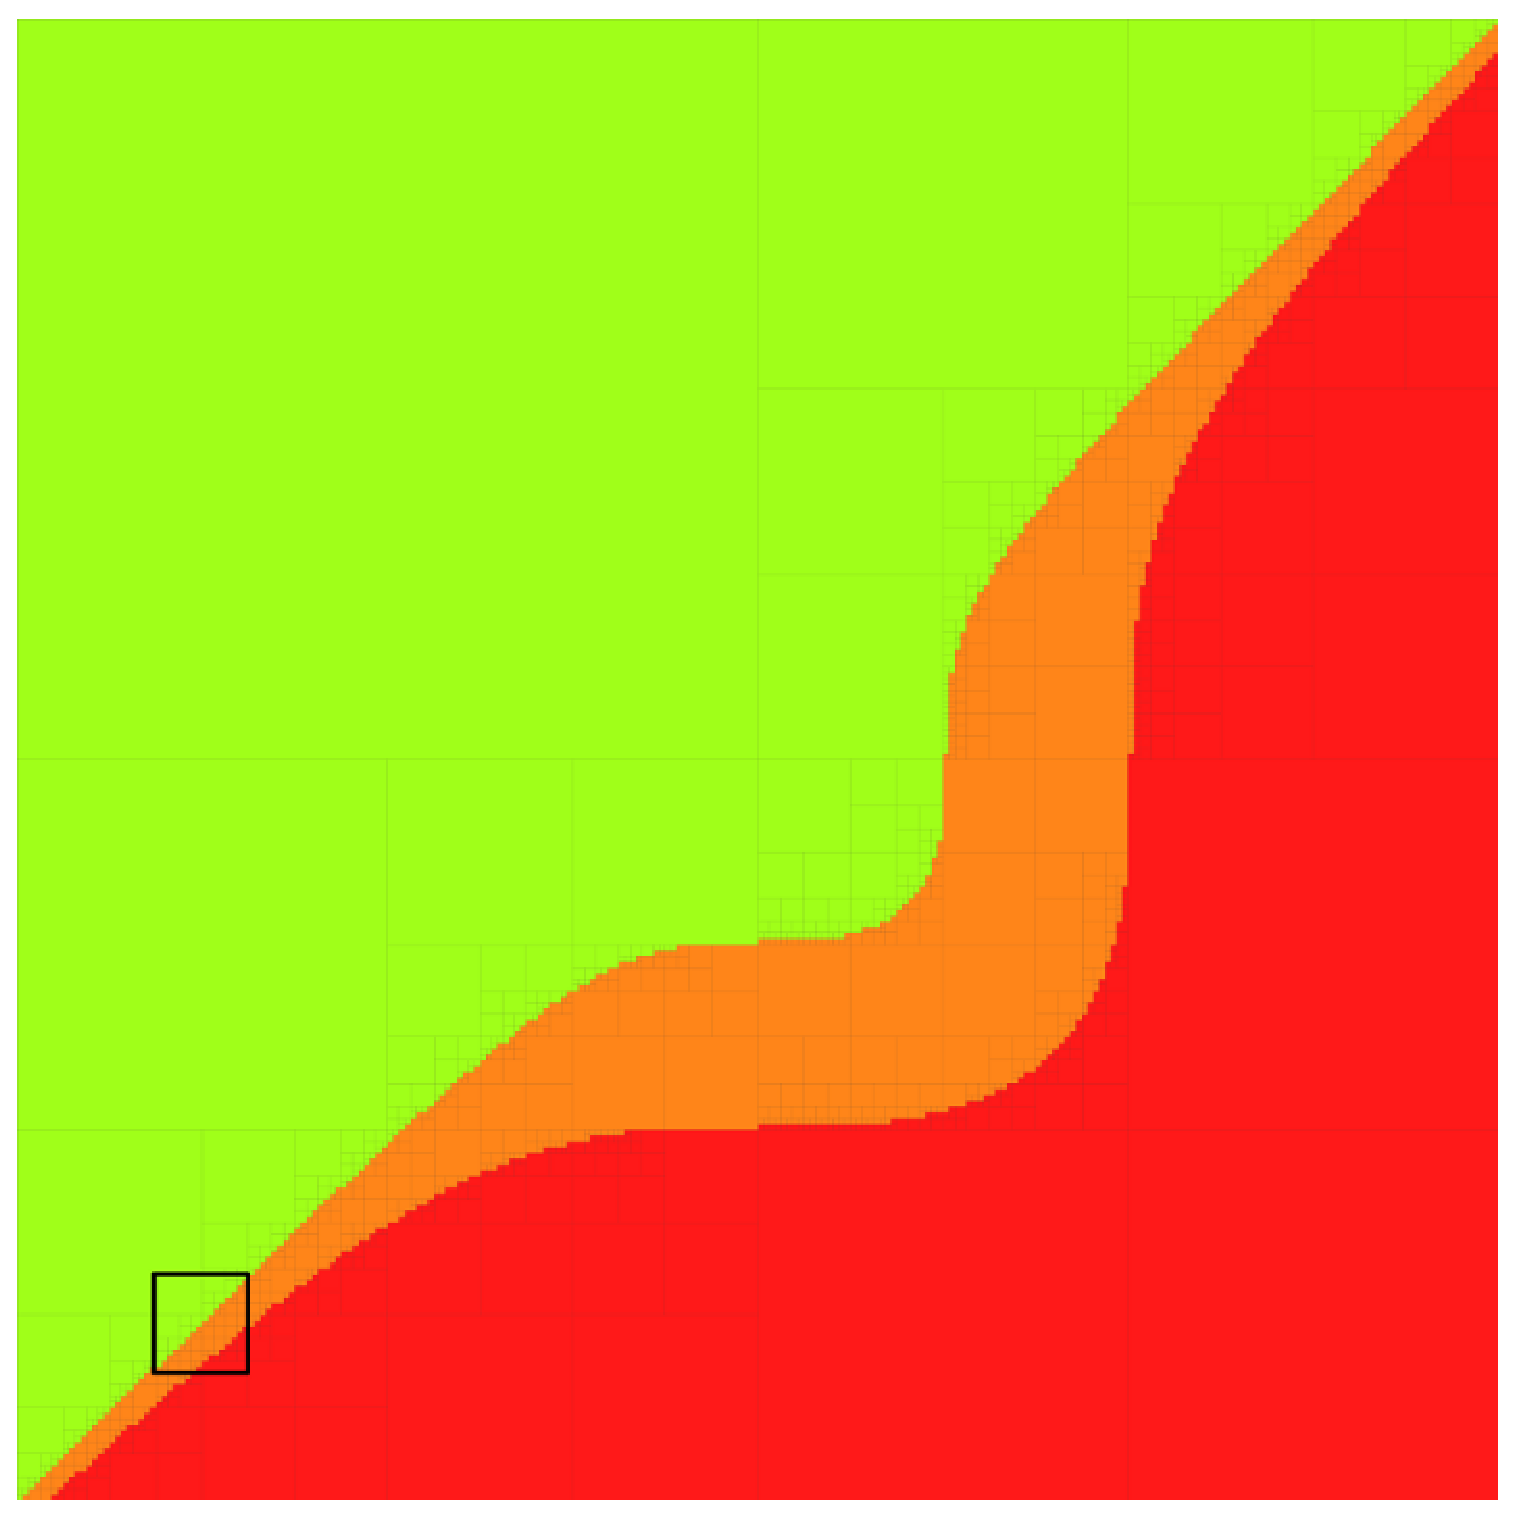
\includegraphics[height=0.3\textwidth]{Images/hashtree-1.eps}%
}&
\framebox{%
  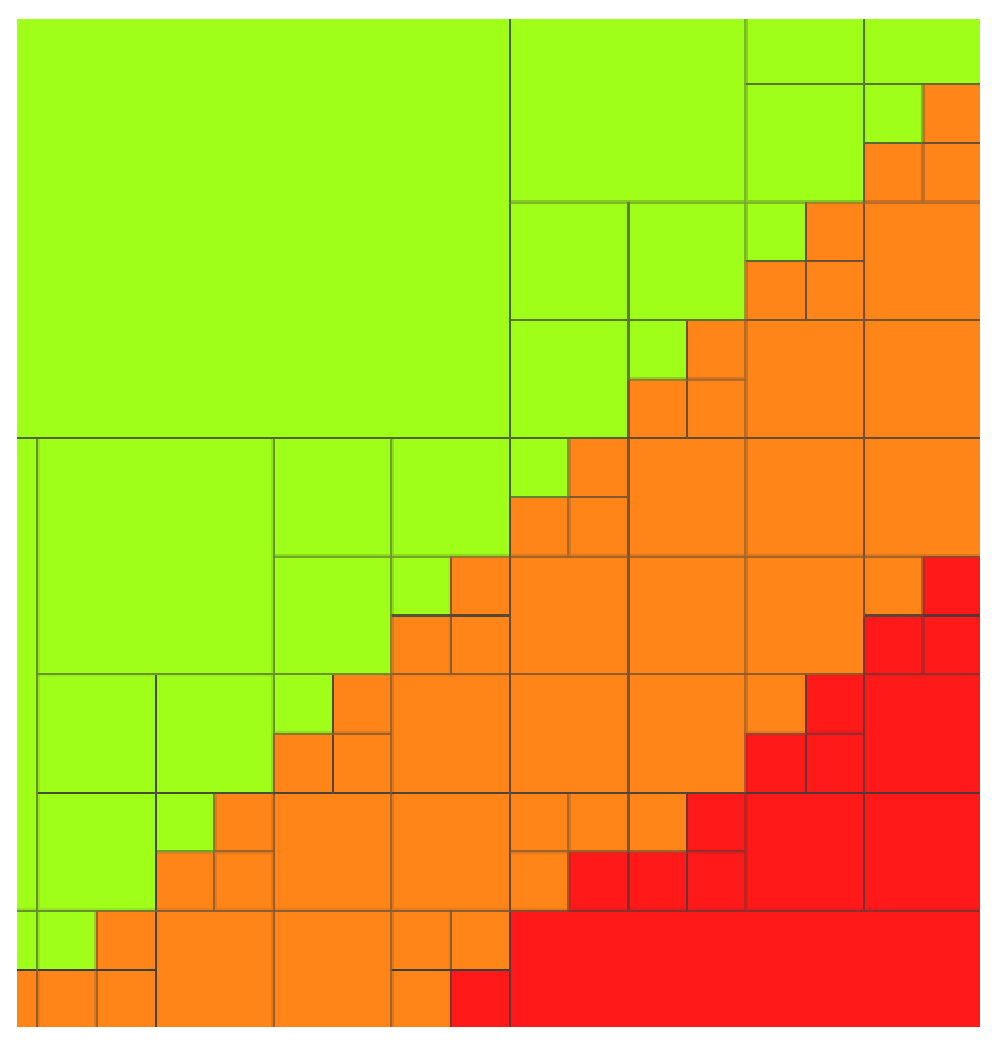
\includegraphics[height=0.3\textwidth]{Images/hashtree-2.eps}%
}\\
\end{tabular}
\end{center}
\end{minipage}
\end{colonne}
\hfill
%-------------------------------------------------------------------------------
%Partie Droite
%-------------------------------------------------------------------------------
\begin{colonne}{0.32}

\begin{minipage}[t]{\textwidth}


%\vskip -4cm
\subsection{Digital (Rosenfeld's) topology}
\begin{itemize}
\item digital topologies, connected components, borders, simple points, homotopic thinning
\end{itemize}

\begin{tabular}{ccc}
  \multirow{2}{*}{
    \begin{minipage}{0.27\textwidth}
      \framebox{%
        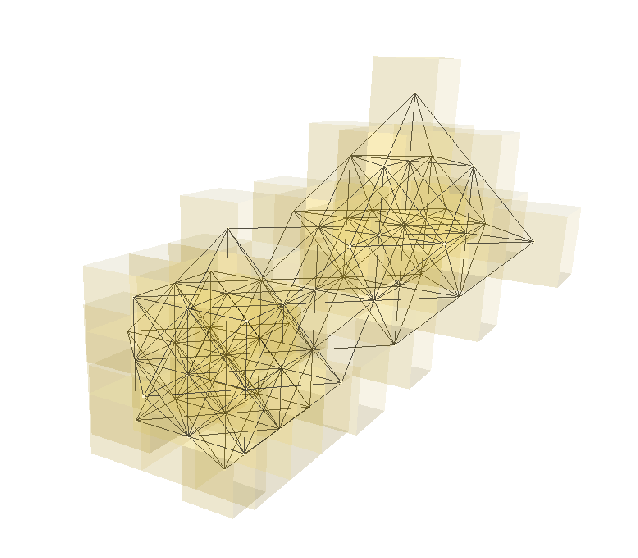
\includegraphics[height=\textwidth]{Images/object-3d-18-6.eps}%
      }
    \end{minipage}
  }&
  \multirow{2}{*}{
    \framebox{%
      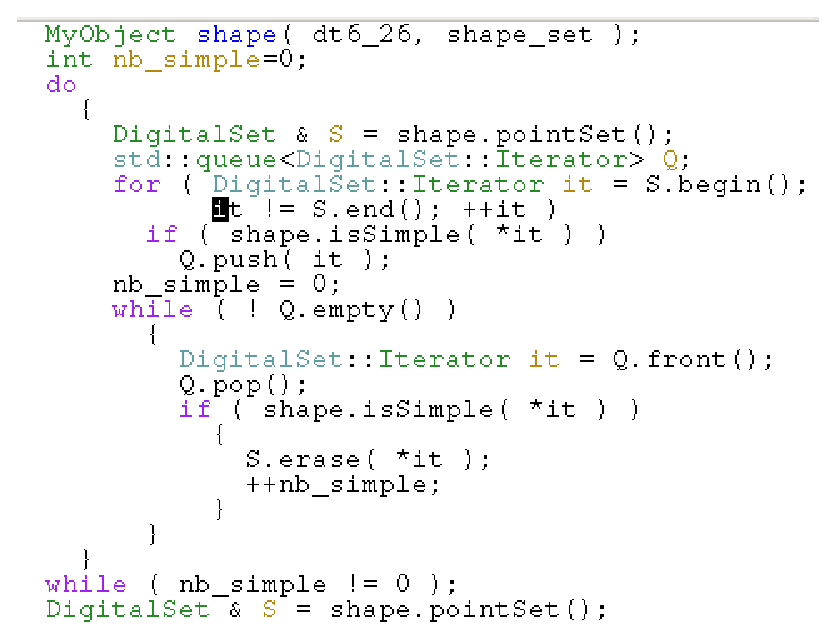
\includegraphics[trim= 0 0 0 1cm , clip, height=0.27\textwidth]{Images/code-thinning.eps}%
    }
  }&
  \raisebox{-4cm}{
    \framebox{%
      \includegraphics[width=0.15\textwidth]{Images/thinning-2d.eps}%
    }
  }\\
  &
  &
  \raisebox{-4cm}{
    \framebox{%
      \includegraphics[width=0.15\textwidth]{Images/thinning-3d.eps}%
    }
}
  \\
%% \begin{minipage}{0.25\textwidth}
%% \vspace{-3cm}
%% \framebox{%
%%   \includegraphics[width=0.7\textwidth]{Images/thinning-2d.eps}%
%% }\\
%% \framebox{%
%%   \includegraphics[width=0.7\textwidth]{Images/thinning-3d.eps}%
%% }
%% \end{minipage}
\end{tabular}

\subsection{Geometry analysis}
\begin{itemize}
\item 2d contours, primitives, DSL and DSS, decomposition, tangential cover
\end{itemize}

\begin{tabular}{cc}
\framebox{%
%  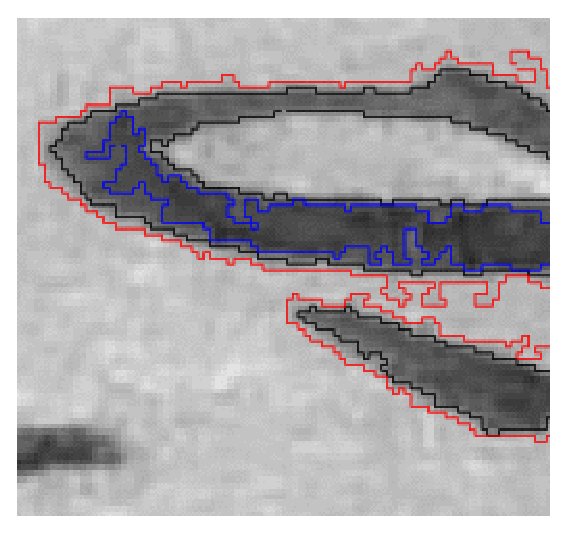
\includegraphics[height=0.2\textwidth]{Images/contourS1-2.eps}%
  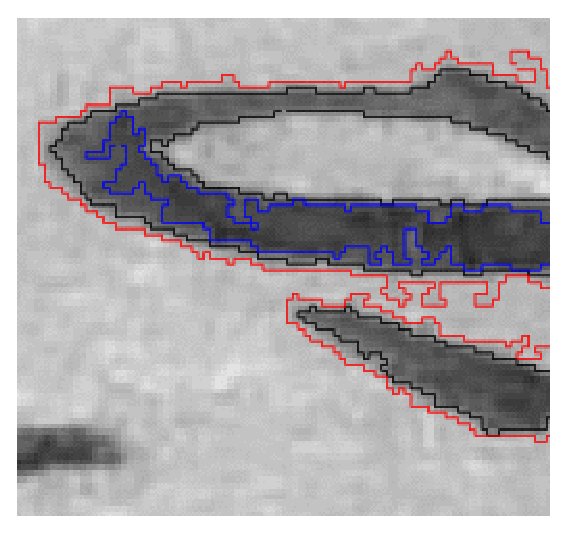
\includegraphics[trim= 1cm 1.5cm 0cm 0.5cm, clip, height=0.2\textwidth]{Images/contourS1-2.eps}%
}&
\framebox{%
  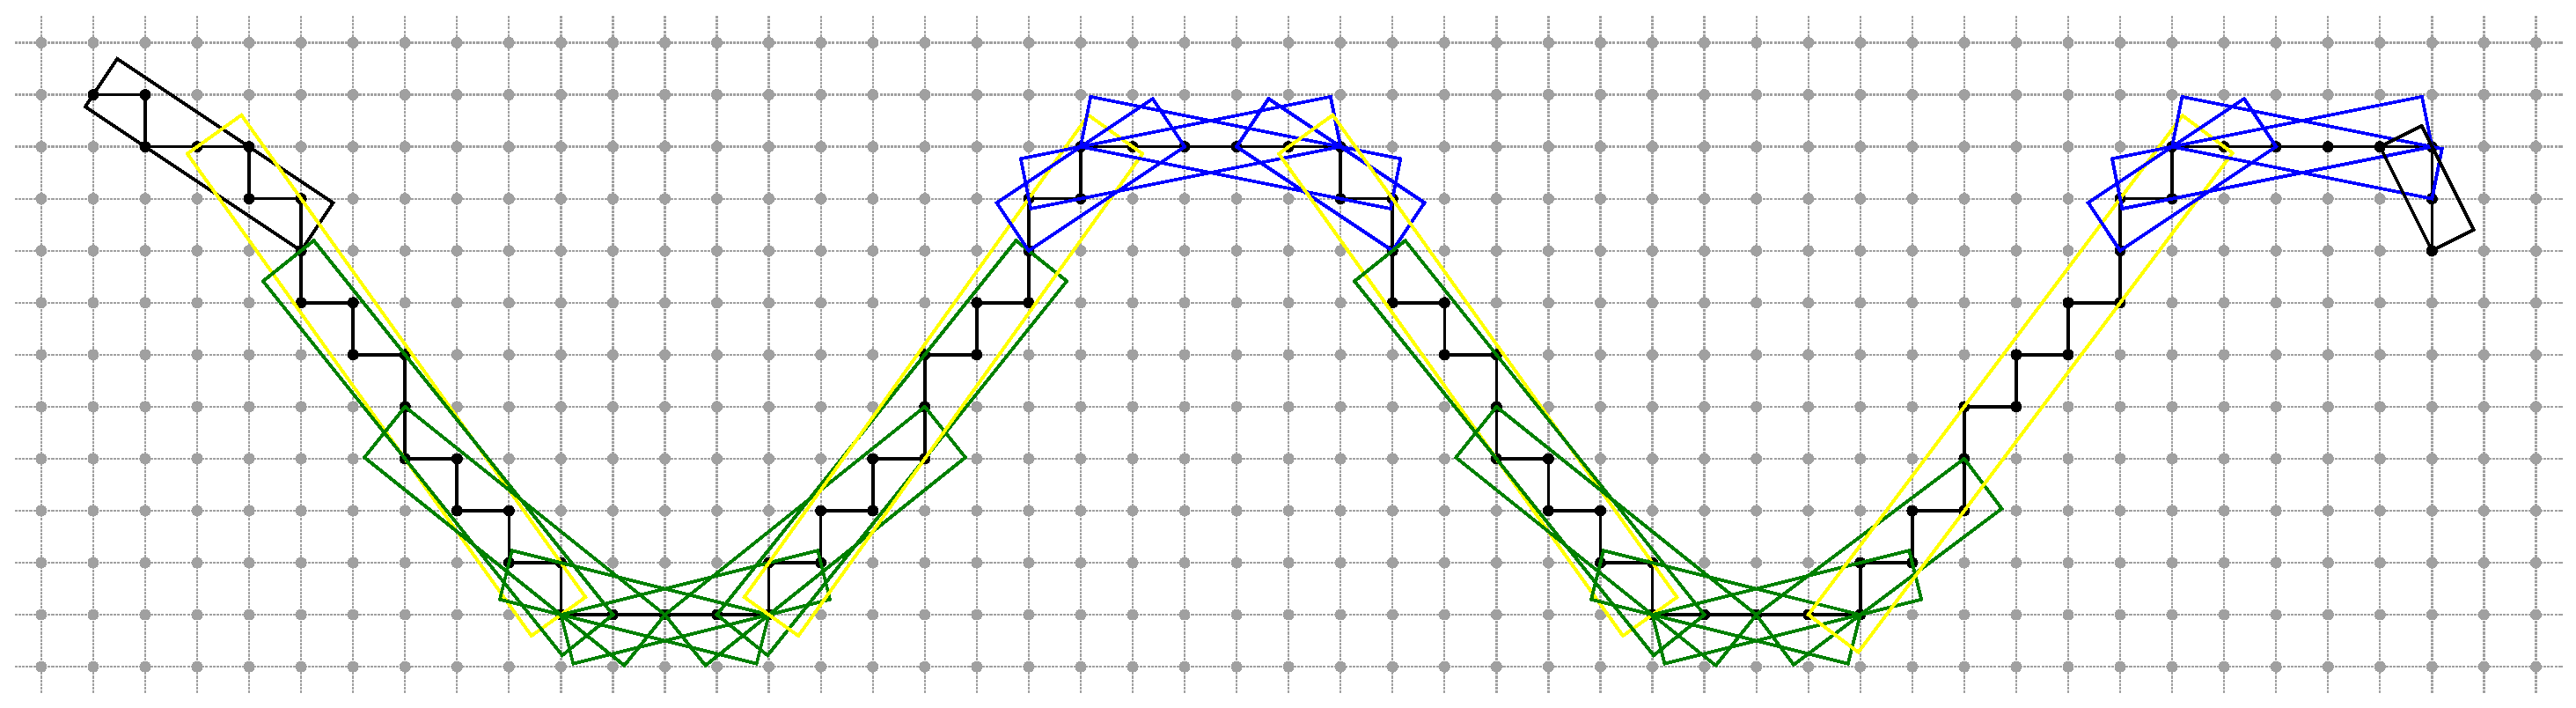
\includegraphics[height=0.17\textwidth]{Images/convex-and-concave-parts.eps}%
}\\
\end{tabular}

\begin{itemize}
\item $n$D volumetric distance transforms
\end{itemize}
\begin{center}
\begin{tabular}{cccc}
\framebox{%
  \includegraphics[height=0.2\textwidth]{Images/dt-2d.eps}%
}&
\framebox{%
  \includegraphics[height=0.2\textwidth]{Images/edt-2d.eps}%
}&
\framebox{%
%  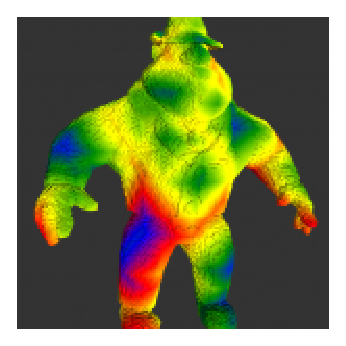
\includegraphics[height=0.2\textwidth]{Images/al-dt.eps}%
  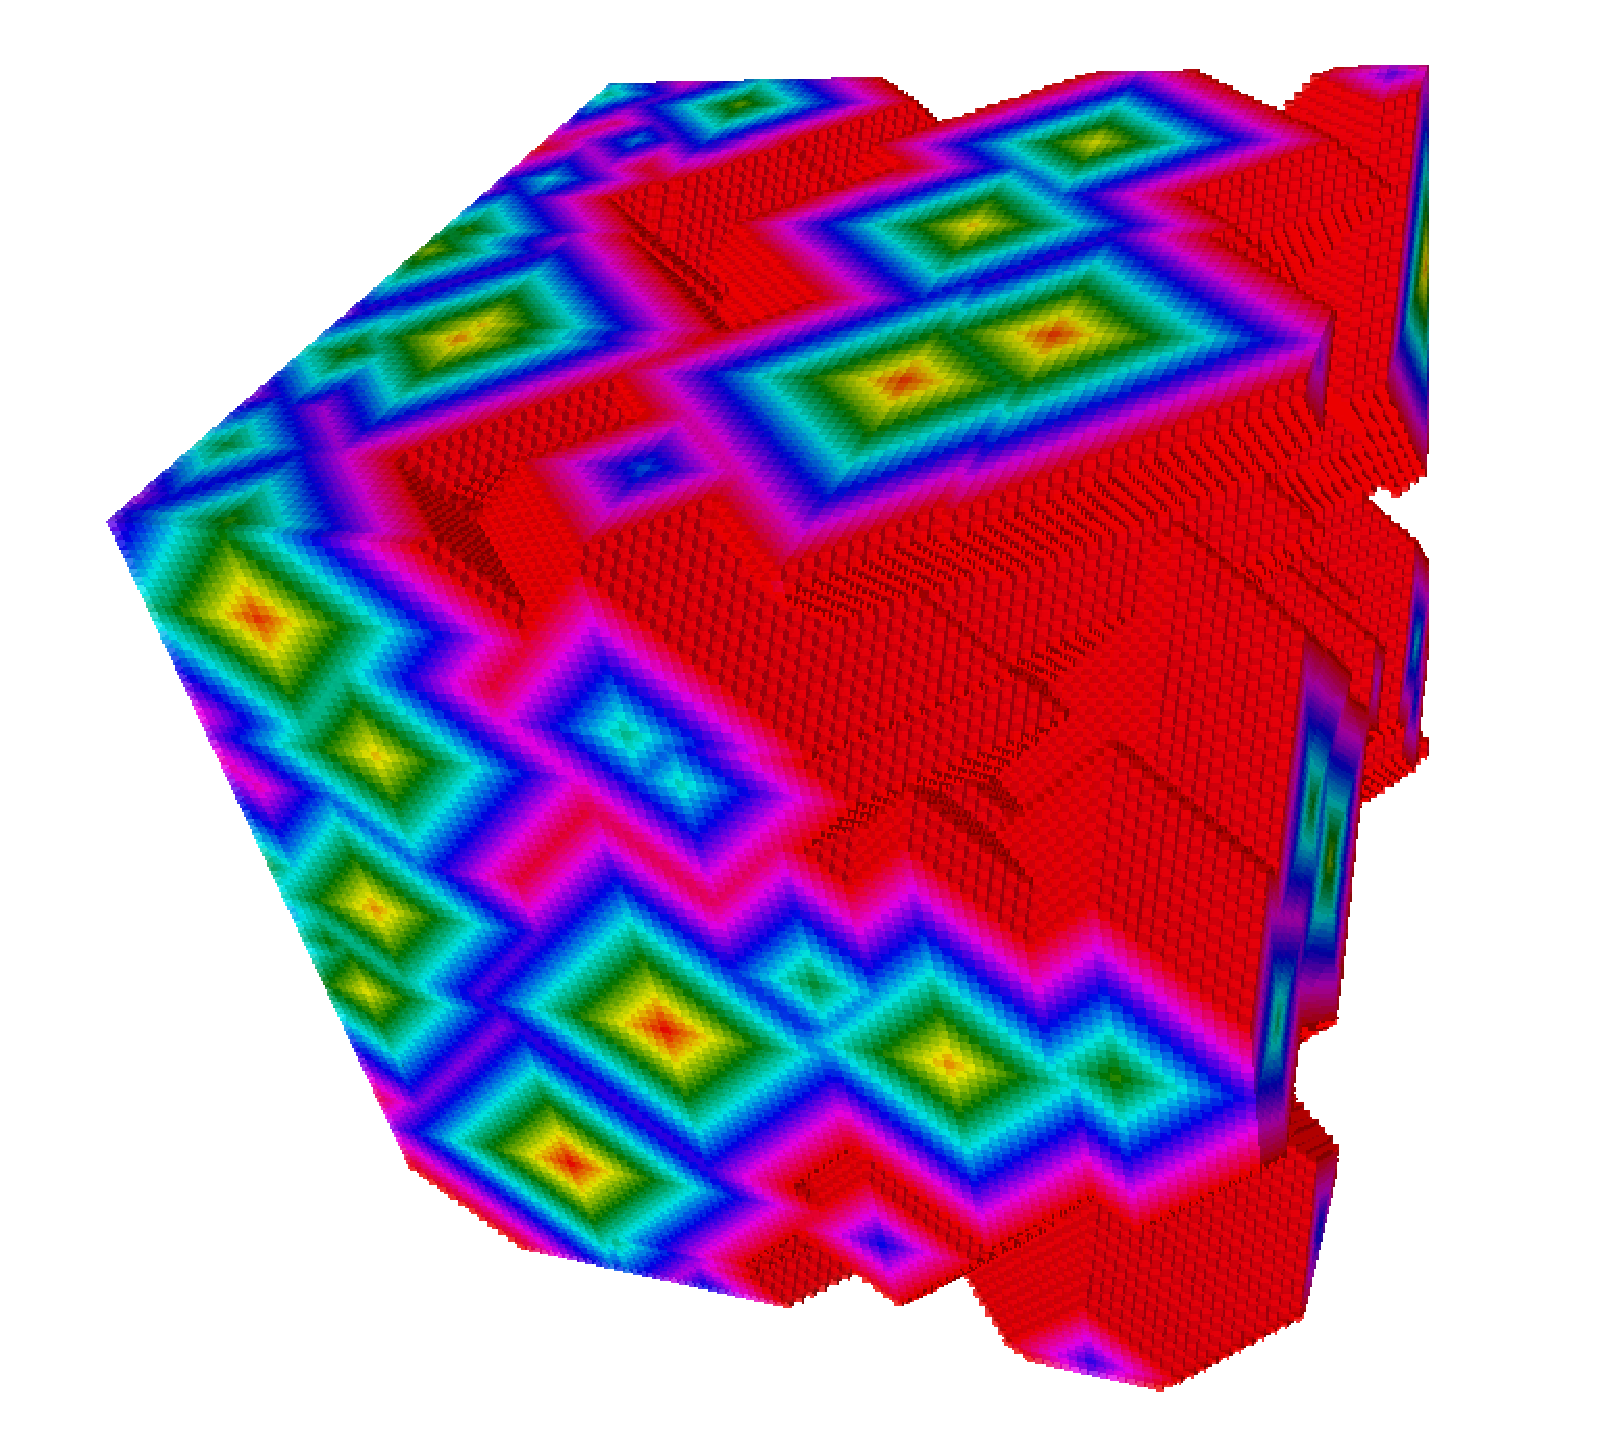
\includegraphics[height=0.2\textwidth]{Images/dt3dl1.eps}%
}&
\framebox{%
%  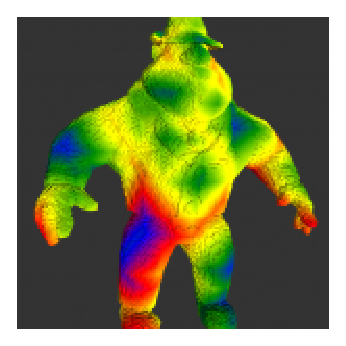
\includegraphics[height=0.2\textwidth]{Images/al-dt.eps}%
  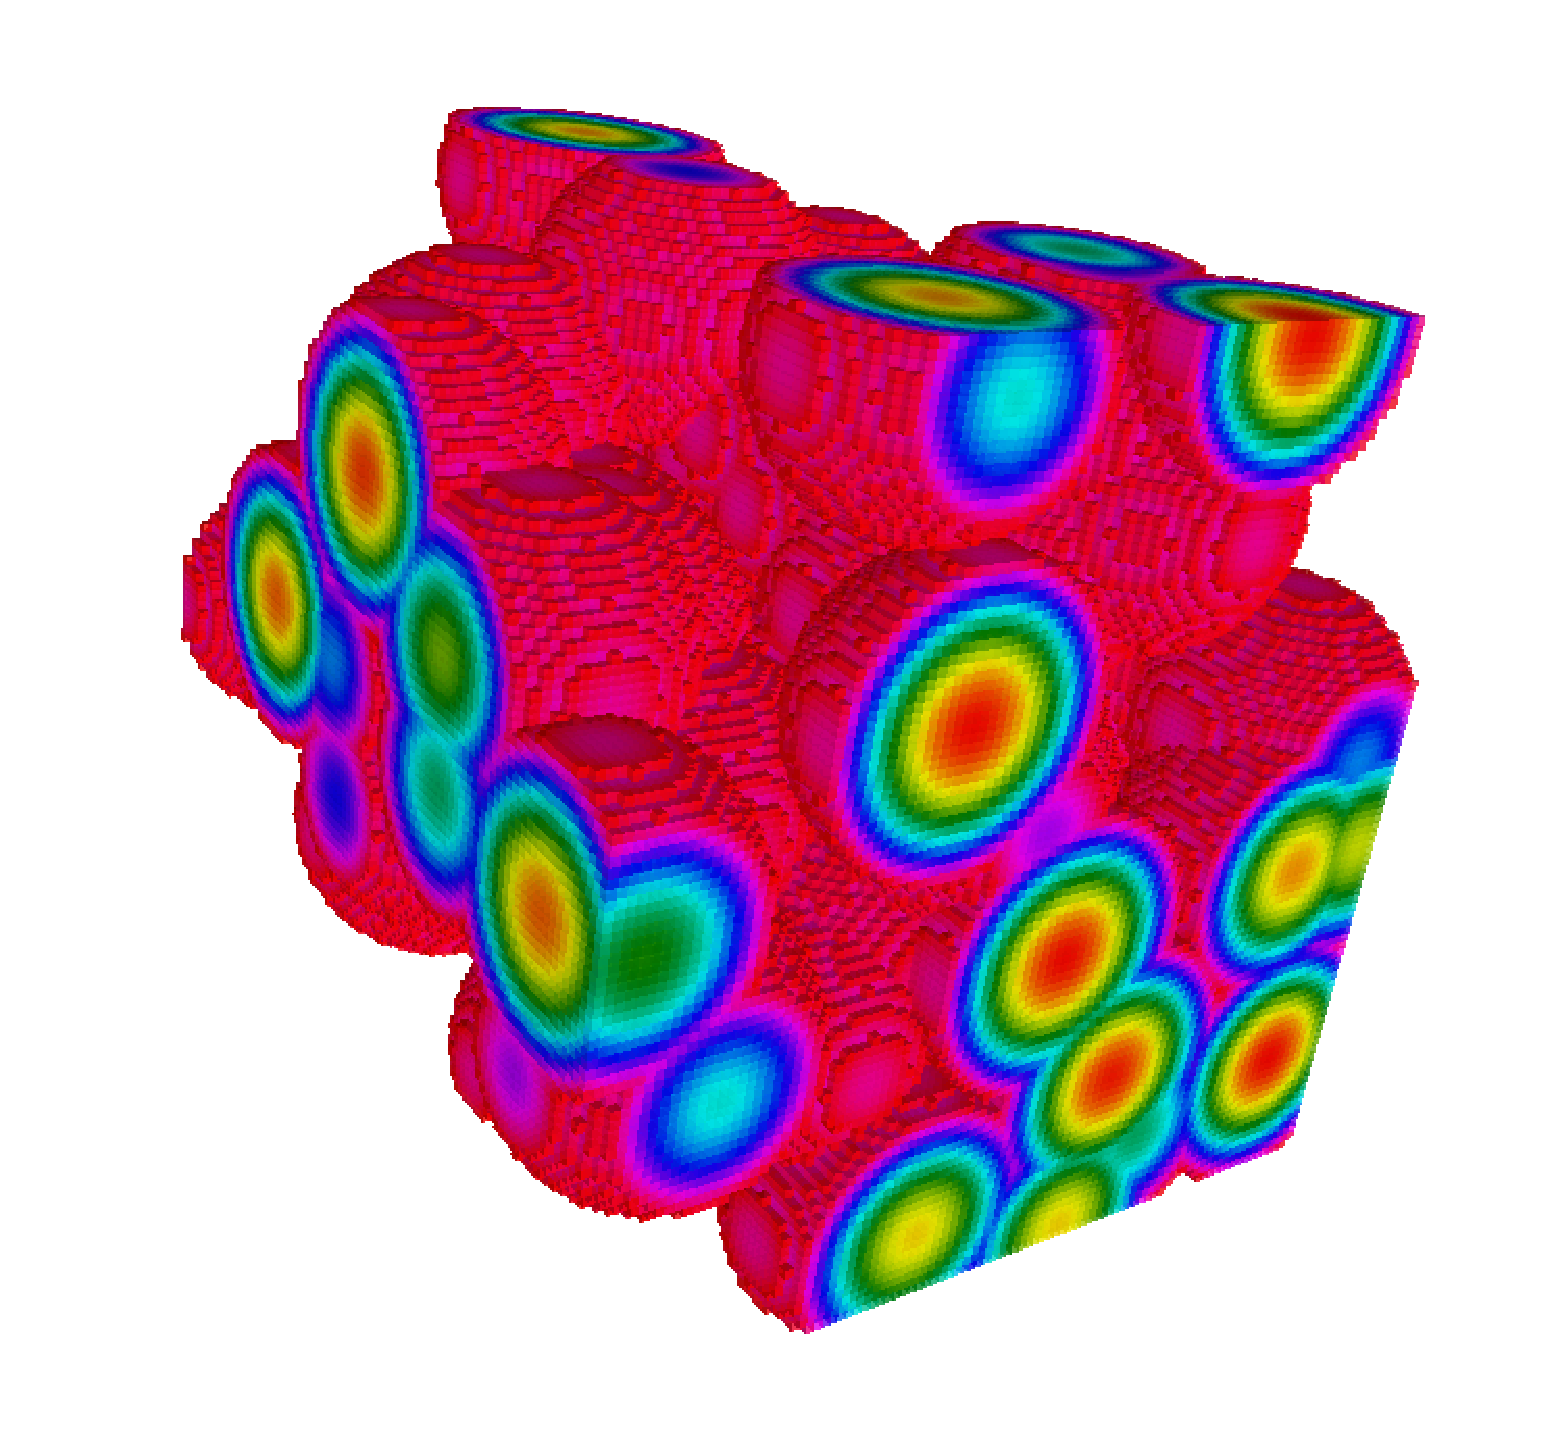
\includegraphics[height=0.2\textwidth]{Images/dt3d.eps}%
}\\
\end{tabular}
\end{center}



\subsection{Additional features}

\begin{itemize}
\item simple 2D vector display and export with stream mechanism
\item 3D viewer with stream mechanism based on QGLviewer ({\color{red}
  New in 0.3})
\item image, volumes import/export
\item grid or interpixel topology, cells, digital surfaces, surface
  tracking ({\color{red} New in 0.3})
\end{itemize}

\begin{center}
\begin{tabular}{ccc}
\framebox{%
  
\includegraphics[height=0.2\textwidth]{Images/lobster.eps}%
}&
\framebox{%
  
\includegraphics[height=0.2\textwidth]{Images/border-extraction-3d.eps}%
}&
\begin{minipage}[b]{0.5\textwidth}
  \begin{itemize}
    \item Forge (trac), unit tests, cmake/ctest/cdash, mailing lists
    \item User and developer documentation (doxygen)
    \item Cross-platform (Linux, MacOS, Windows)
    \item {\color{magenta} Join DGtal !}
  \end{itemize}
\end{minipage}
\\
\end{tabular}
\end{center}

\end{minipage}
%% \begin{minipage}{\textwidth}
%% \bigskip
%% \bibliographystyle{plain}
%% \small{\bibliography{posterDGCI}}

%% \end{minipage}













\end{colonne}



\end{poster}

\end{document}
